\begin{bclogo}[couleur = gray!20, arrondi = 0.2, logo=\bcattention]{Incremental code}
As for last session, we provide you with a "golden version" of the project at this point. If you are not sure about the correctness of your implementation, download \texttt{p2b.patch} from Moodle and apply it to your repository. Note that the patches are incremental, meaning that you must apply \texttt{p2a.patch} (if not already done), then \texttt{p2b.patch} on top of it.
\end{bclogo}

\section{Measuring the execution time}

In the first part of this session, you will measure the execution time of the function \texttt{melvec\_compute()}, using two different methods.

\subsection{Measuring the time elapsed on the oscilloscope}

The first technique is to set the voltage high or low on a GPIO pin to signal the beginning and the end of a task. It is pretty similar to blinking an LED, but it enables accurate timing measurements through the oscilloscope.

\begin{enumerate}
	\item Open STM32CubeMX. In the pinout view, locate the pin \textbf{PB11} near the lower-right corner as in \autoref{fig:gpout-cubemx}. Click on the pin and set its function to \textbf{GPIO\_Output}. Rename the pin \textbf{GPOUT} by \textbf{right-clicking} it, then \textbf{Enter User Label}. Don't forget to regenerate the code ;
\begin{figure}[H]
    \centering
    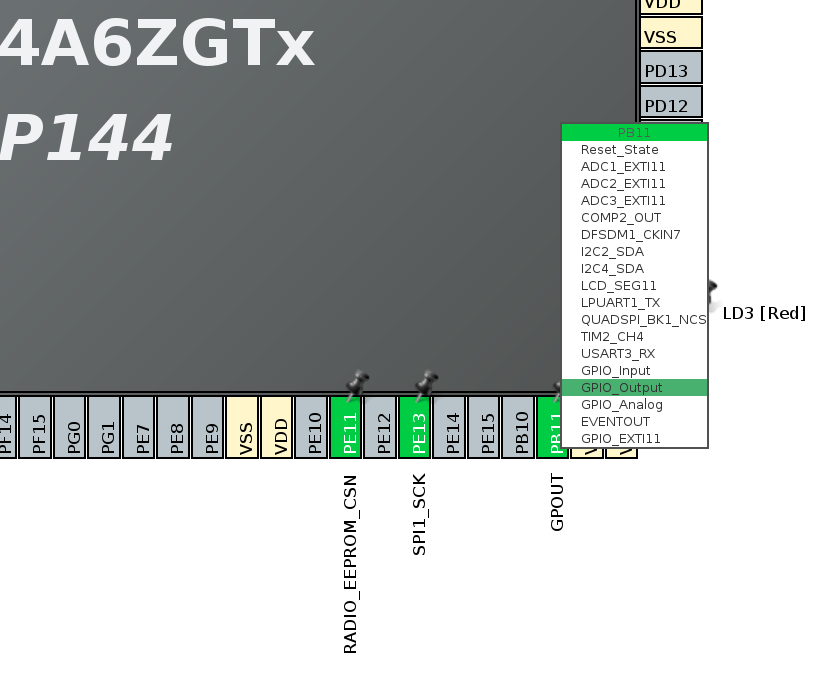
\includegraphics[width=.65\textwidth]{figures/gpout_cubemx.png}
    \caption{PB11 configuration as GPOUT in STM32CubeMX.}
    \label{fig:gpout-cubemx}
\end{figure}
	\item In the main loop, set GPOUT high before calling \texttt{melvec\_compute()}, then set it low right after. \textit{Hint:} The HAL functions you need to call are the same as the ones you used to light on and off the LED, but this time you must use the right pin user label defined in \texttt{main.h} : \texttt{GPOUT\_GPIO\_Port} and \texttt{GPOUT\_Pin} ;
	\item Connect the channel 1 of the ADALM2000 oscilloscope to the MCU in order to probe GPOUT. Three pins must be connected : \textbf{GND} and \textbf{1-} of the ADALM to any ground pin on the MCU (there are many available on the green and white boards, look for \textit{GND} labels), and \textbf{1+} to \textbf{PB11} as in \autoref{fig:adalm} ;
\begin{figure}[H]
    \centering
    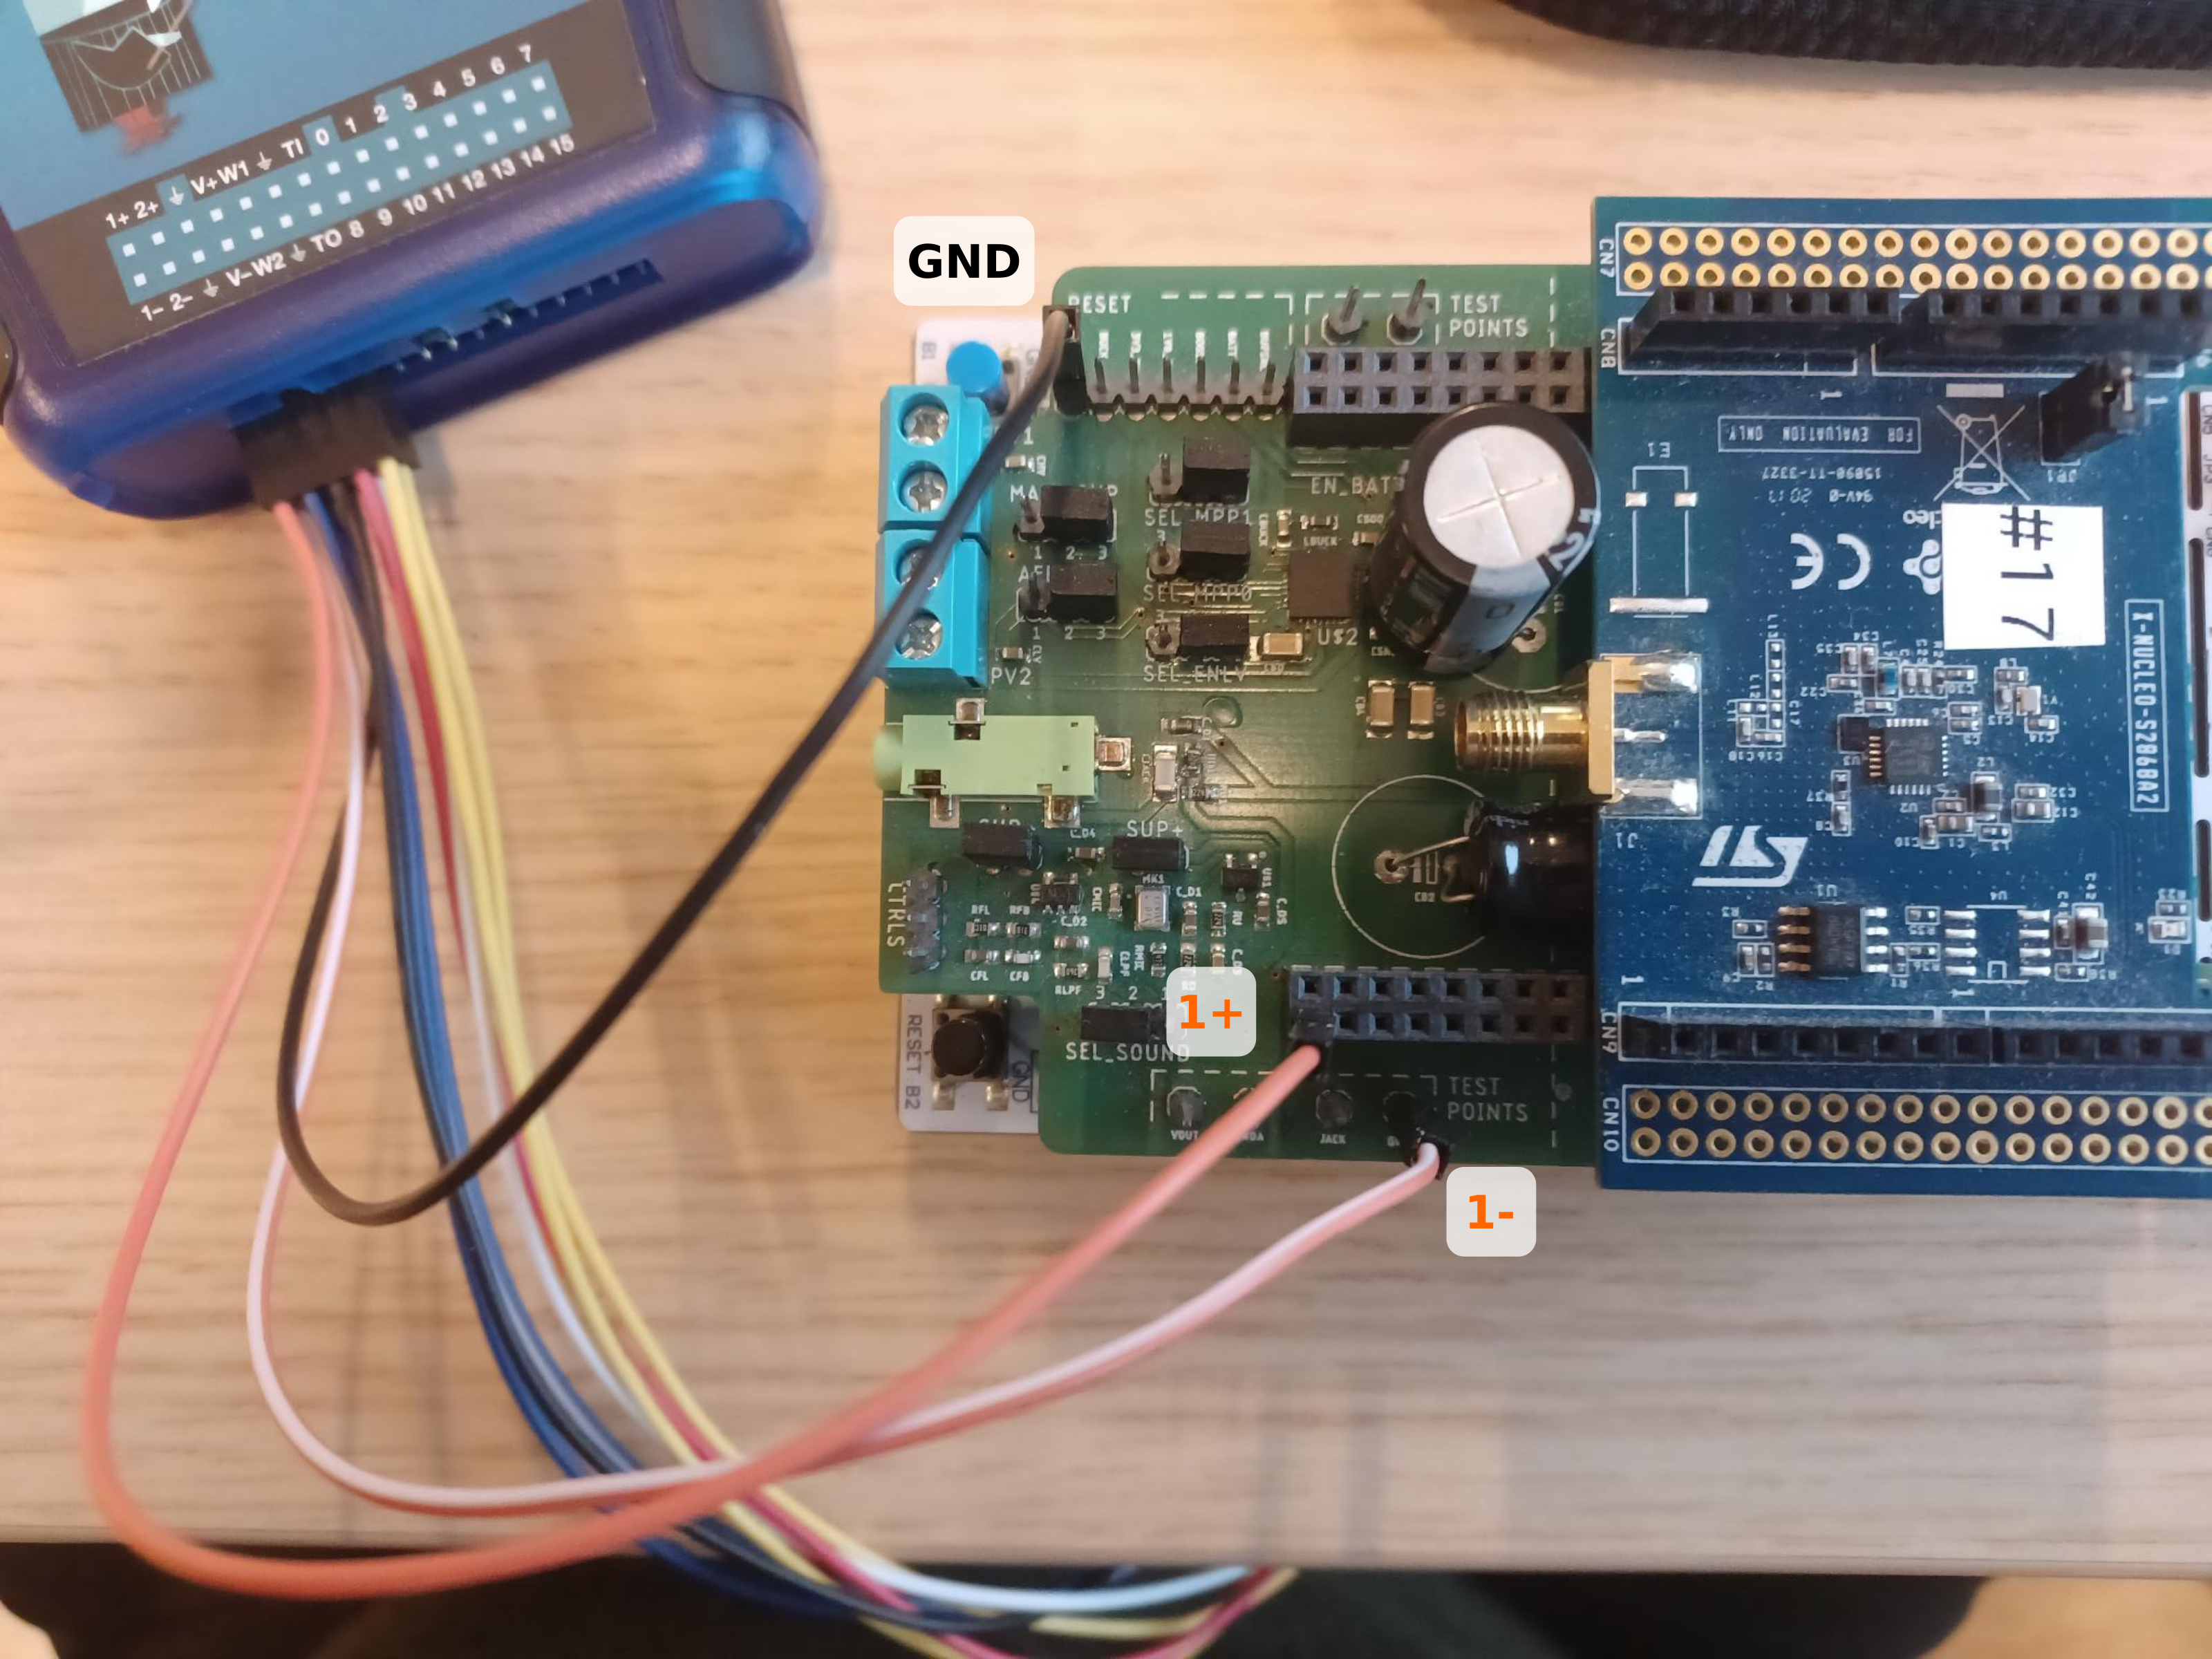
\includegraphics[width=.65\textwidth]{figures/adalm.png}
    \caption{ADALM2000 oscilloscope channel 1 connection to GPOUT.}
    \label{fig:adalm}
\end{figure}
	\item Open \textbf{Scopy} and observe the GPOUT trace while acquiring samples and computing melvectors. \textit{Hint:} Set up a trigger at around VDD/2 and use the single acquisition mode of the oscilloscope. Make use of cursors for accurate timing measurements.
\end{enumerate}

\begin{bclogo}[couleur = gray!20, arrondi = 0.2, logo=\bcquestion]{Computation and acquisition timings}
Can you identify the beginning and end of each mel-vector computation on the GPOUT trace ? How much time is required by the CPU to execute \texttt{melvec\_compute()} ? How much time does the acquisition of one sample buffer take ? Does it match your expectations ?
\end{bclogo}

\begin{bclogo}[couleur = gray!20, arrondi = 0.2, logo=\bcinfo]{Nucleo board pinout}
In the technical resources on Moodle, you can find the \textbf{Nucleo-L4A6ZG user manual} that details the features of the MCU board we use in this project. In page 33, you will find the expansion connector's pinout that shows where to locate PB11 or any other pin. Notice how the green custom board is stacked on top of the MCU board, with the connectors aligned.
\end{bclogo}

\subsection{Counting CPU cycles}

Another technique to measure the execution time is to count the CPU cycles elapsed during some function execution. In \texttt{utils.c}
/\texttt{.h}, we provide you with a function that starts a cycle counter, and another one that stops it and prints the count.
\begin{enumerate}
	\item For now, the functions are not compiled due to the value of the macro \texttt{PERF\_COUNT}. In \texttt{config.h} set that macro to \textbf{1} to enable the performance counters ;
	\item In \texttt{computation.c}, enclose each step of the computation within the counter functions ;
\begin{lstlisting}[columns=fullflexible]
start_cycle_count();
// The function to measure
stop_cycle_count("step XX");
\end{lstlisting}
	\item Build and flash the program, then retrieve the measurements from the console of \texttt{uart-reader}.
\end{enumerate}

\begin{bclogo}[couleur = gray!20, arrondi = 0.2, logo=\bcquestion]{Cycle count of each computation step}
What is the number of cycles taken by each step of the mel-vector computation ? What is (are) the bottleneck(s), i.e. the steps that require the highest number of cycle and that would thus be the most interesting to optimise ? If you already have some ideas on how to reduce the total number of cycles, write them down as it will be useful later in the project.
\end{bclogo}

\begin{bclogo}[couleur = gray!20, arrondi = 0.2, logo=\bcinfo]{Cycle counter and interrupts}
The cycle counter is a special register in the DWT unit (Digital Watchdog Trigger) of the MCU. It is incremented at each clock cycle and thus contains the cycle count from its last reset at any time. The functions we provide you with are simply wrappers around that counter.

Note that if some interrupt is executed during the measured function, the counter makes no difference and the count is thus higher. This is the reason why the count is slightly different at each iteration, but the difference is negligeable in our case.
\end{bclogo}

\begin{bclogo}[couleur = gray!20, arrondi = 0.2, logo=\bcinfo]{Computational complexity}
The computational complexity of each step of \texttt{melvec\_compute()} is indicated in \texttt{acquisition.c}, using the Big O notation (e.g. $O(n)$, $O(\log{n})$, etc.). It describes the asymptotic growth rate of the execution time of a function with its input size $n$. In our case, $n$ is the number of samples in the input buffer.

It is interesting to keep the complexity in mind when thinking about computational bottlenecks, as you may want to modify the mel-vector parameters and thus affect the computation time requirements later in the project.
\end{bclogo}

\begin{bclogo}[couleur = gray!20, arrondi = 0.2, logo=\bcattention]{\texttt{printf}'s take time !}
While setting a GPIO high or low only takes a handful of cycles, printing strings through UART takes a lot of time. Be aware that you greatly modify the execution time when adding \texttt{printf}'s, including the one in the cycle counter function.

You can test it yourself : count the number of cycles required to set GPOUT high, then the one to print some string. You can also observe it in the GPOUT trace on the oscilloscope : how much time does the mel-vector computation take when counting and printing the cycles of each step ?

Do not hesitate to disable the cycle counters and the debug prints altogether using the dedicated macros in \texttt{config.h} when they are not needed.
\end{bclogo}

\begin{bclogo}[couleur = gray!20, arrondi = 0.2, logo=\bcquestion]{Timing constraint}
\begin{itemize}
	\item What is the timing constraint associated with the acquisition of samples and the computation of mel-vectors ? Which condition needs to be respected in order to compute correct mel-vectors ?
	\item What happens if you decrease or increase the CPU clock frequency while keeping the same sampling (timer) frequency ? How does the number of cycles taken by the function \texttt{melvec\_compute()} evolve ? What about the time required by the computation ? At this point, what is the minimum CPU clock frequency you could set without violating the timing constraint ?
\end{itemize}
\end{bclogo}

\section{Optimising the compilation}

The GCC compiler can be configured to optimise the binary it generates based on the C source files. Until now, you have compiled the code using the \textbf{Debug} configuration which is not optimised : nearly every line of code translates to one or several CPU instructions. It is direct, easy to understand and essential to debug the code in real time as we did in P2a.

You will now compile the code with some optimisations and observe their impact.
\begin{enumerate}
	\item Open the properties window in \textbf{Project} $\rightarrow$ \textbf{Properties} ; 
	\item In the left pane, go to \textbf{C/C++ Build} $\rightarrow$ \textbf{Settings}. Then in \textbf{Tool Settings}, go to \textbf{MCU/MPU GCC Compiler} $\rightarrow$ \textbf{Optimization}. There you can choose the \textbf{Optimization level} from the drop menu.
	\item Note that the active configuration in the panel header is \textbf{Debug} and that no optimisation is currently configured. Select \textbf{Release} as the active configuration and set the level to \textbf{Optimize (-O1)}. Click on the green button \textbf{Apply and close} ;
	\item Click on the arrow next to the \textbf{Build} hammer-shaped button and verify that \textbf{Release} is indeed active, then build the project by clicking it ;
	\item Click now on the arrow next to the \textbf{Flash} green triangle button, then \textbf{Run As} $\rightarrow$ \textbf{STM32 C/C++ Application}. In the window that popped up, choose the binary located in the \textbf{Release} folder. Keep the default parameters for the new launch configuration and click \textbf{Ok}, this will flash the MCU in \textbf{Release} mode. The flash button drop menu now shows two configurations, you can use one or the other as you seem fit.
\end{enumerate}

Measure the execution time of that optimised program using the same techniques as before. Observe and explain the changes.

\begin{bclogo}[couleur = gray!20, arrondi = 0.2, logo=\bcinfo]{Optimisation levels and techniques}
Optimising the compilation is a tradeoff between compilation effort, binary program size and execution time. Different optimisation techniques are used by the compiler, such as \textit{loop unrolling} that increases the code size and accelerates its execution.

Refer to the official GCC manual to know more about the levels and the techniques employed : \url{https://gcc.gnu.org/onlinedocs/gcc/Optimize-Options.html}.%\footnote{These optimisations happen at the compiler level, and each file is compiled individually. Since optimization is based on gathering information on the code and how it is used, this limited (file-level) view may lead to missed optimization opportunities. Link-time optimization (LTO) is a technique that enables project-level view for optimizations and that you might want to use at some stage of your project. To add such custom compiler and linker flags, use the \textbf{Miscellaneous} section of the Compiler/Linker settings.}
\end{bclogo}

\begin{bclogo}[couleur = gray!20, arrondi = 0.2, logo=\bcquestion]{Knowing the binary program size}
In the lower-right panel of STM32CubeIDE, there is a tab named \textbf{Build Analyzer} that provides information about the memory (RAM and flash) footprint of the compiled program. You may need to refresh it using the double-arrows button.

\begin{itemize}
	\item What is stored in the RAM memory, and what is stored in the flash memory ? Are they volatile or non-volatile memories ? What is written during the flash procedure and what is written at runtime ?
	\item What is the memory footprint before and after using the compiler optimisations ?
	\item What parameters or configuration would impact both memory footprints ? Do you consider one and/or the other as a bottleneck of your system ?
\end{itemize}
\end{bclogo}

\begin{bclogo}[couleur = gray!20, arrondi = 0.2, logo=\bcquestion]{Optimisation level tradeoff}
\begin{itemize}
\item What are the different optimisation levels you can select ? What is the impact of each of them on the three metrics of the tradeoff ?
\item Quantify the impact of some interesting optimisation levels by measuring the execution time and the memory footprint associated with them.
\item Which optimisation level would you choose regarding the constraints of your system ?
\end{itemize}
\end{bclogo}
